\chapter{Fundamentação Teórica}


\section{Arquiteturas Paralelas}
Até a última década, o desempenho sobre computadores escalava de acordo com o aumento da frequência dos processadores. Contudo, de acordo com a equação~\eqref{eq:power} pode-se perceber que a potência aumenta, proporcionalmente, ao aumento da frequência. Portanto, o aumento do desempenho encontrou uma barreira de consumo de energia. Desta forma, tornou-se necessário uma nova abordagem para aumentar o desempenho dos computadores, uma solução seria o paralelismo dos algoritmos sobre as \textit{threads} ou \textit{cores} de uma \cpu.

\begin{equation}\label{eq:power}
	P = C \times V^2 \times F
\end{equation}

Existem diversos tipos de arquiteturas que proporcionam ao desenvolvedor uma abordagem paralela. Multiprocessadores são arquiteturas que fornecem vários núcleos de processamento em uma máquina e a comunicação entre os núcleos é feita através da memória compartilhada, contudo este modelo traz dificuldades em relação à organização e particionamento de dados entre núcleos. Devido ao espaço limitado em \textit{chip}, o aumento do número de núcleos nessa arquitetura pode se tornar inviável, portanto, arquiteturas multicomputadas são utilizadas, onde temos várias máquinas, sendo, geralmente, multiprocessadas, interligadas para fornecer um maior poder de processamento. A comunicação entre cada \textit{cluster}, isto é, cada nó na rede de computadores utiliza distribuição de dados e sincronizações, como não temos compartilhamento de memória entre os nós de processamento, o desenvolvimento de código para essa arquitetura é mais complicada, pois existem vários fatores à serem avaliados pelo desenvolvedor. Na próxima seção serão abordadas as dificuldades e implementação de cada modelo.

%Arquiteturas paralelas: multicomputadores, multiprocessadores, compartilhamento de memória e distribuição de dados.
%Programação paralela: uso de apis, dificuldades. POSIX, MPI...


\section{Programação Paralela}
O desenvolvimento de aplicações são, geralmente, implementadas de forma sequêncial, isto é, um conjunto serializado de instruções que será executado sobre uma \cpu. Por outro lado, a computação paralela ou distribuída efetua o processamento de instruções sobre múltiplos elementos de processamento. Dentre esses elementos, pode-se ter várias \cpu{}s (multicomputado) ou várias \textit{threads} dentro da mesma \cpu (multiprocessado). O algoritmo que compõe a implementação pode ser dividido em partes menores que podem ser executadas simultâneamente entre os elementos de processamento.
%falar sobre distribuida e paralela.


Computação paralela em uma arquitetura multiprocessada contém diversas dificuldades para o desenvolvimento de código, como: \textbf{(i) dependência de dados:} quando um processo ou \textit{thread} está executando uma parte do código, outra \textit{thread} deve ter os dados atualizados corretamente. Esta dependência pode gerar problemas com o código, como \textit{deadlocks} e \textit{livelocks}. \textit{Deadlocks} são conflitos que ocorrem entre \textit{threads}, quando uma \textit{thread} A precisa de um recurso alocado por uma \textit{thread} B que, por sua vez, precisa de um recurso alocado pela \textit{thread} A, estagnando a execução. \textit{Livelocks} são similares aos \textit{deadlocks}, contudo o estado das \textit{threads} mudam entre si, fazendo com que nenhum deles continue sua execução normalmente. Além disso, dependências geram problemas de sincronização entre \textit{threads}, deixando para o desenvolvedor da aplicação a tarefa de gerenciar corretamente a execução.%...
\textbf{(ii) Condição de Corrida:} uma \textit{thread} escreve sobre uma váriavel ou, mais especificamente, um espaço de memória, enquanto outra \textit{thread} fará alguma operação sobre esse mesmo espaço. Isso pode gerar inconsistências de dados, entre outros problemas.
Mais especificamente, a comunicação em uma arquitetura multiprocessada é feita por uma \api denominada \openMP. A \api é baseada no modelo de programação paralela de memória compartilhada, apresentando uma boa portabilidade e pouco esforço de programação. O modelo de programação utiliza diretivas de compilação e variáveis, tornando possível poucas modificações de código para utilizar outras \textit{threads} na aplicação.

%
% \renewcommand{\lstlistingname}{Código}
% \definecolor{lightgray}{rgb}{0.97,0.97,0.97}
% \definecolor{lightred}{rgb}{1,0.7,0.7}
%
% \lstdefinelanguage{cc}{
%     language     = C++,
%     morekeywords = {Array2D, __parallel__, Mask2D, Stencil2D, pragma, omp, parallel, printf},
% }
%
% \lstset{
% numbers=none,
% stepnumber=1,
% numbersep=-8pt,
% numberstyle=\small\color{black},
% basicstyle=\scriptsize\ttfamily,
% keywordstyle=\color{blue},
% commentstyle=\color{black},
% stringstyle=\color{black},
% numberstyle=\footnotesize\ttfamily\color{black},
% escapeinside={(@}{@)},
% frame=none, %single
% tabsize=2,
% float,
% language=cc, %morecomment=[l][{\color[rgb]{0.1, 0.2, 0.8}}]{},
% %aboveskip=0.1in, % space before the caption
% %belowskip=0.1in, % space after listing
% captionpos=b,
% showstringspaces=false,
% %belowcaptionskip=1\baselineskip,
% %breaklines=true,
% %moredelim=[l][\color{blue}]{\#pragma},
% backgroundcolor=\color{white},
% %xleftmargin=.2\textwidth, xrightmargin=.2\textwidth
% }
%
% \begin{figure}[thp] % the figure provides the caption
% \centering          % which should be centered
% \begin{tabular}{c}
%
% \begin{lstlisting}[]
%     (@\textcolor{blue}{\#}@)pragma omp parallel
%     printf("Hello World!");
% \end{lstlisting}
% \end{tabular}
% \caption*{Exemplo de código OpenMP.}
% \end{figure}
%



Computações distribuídas (arquiteturas multicomputadas) são utilizadas para dissipar melhor a energia entre \textit{clusters}. Mais especificamente, elas utilizam comunicações por troca de mensagens para efetuar a passagem de informações entre processos. Além disso, esse modelo apresenta dificuldades de sincronização entre \textit{clusters} diferentes em uma mesma rede, comunicação, além dos problemas já apresentados sobre a arquitetura multiprocessada, pois cada nó da rede pode possuir uma arquitetura multiprocessada para aumentar o desempenho de aplicações.
Devido à característica de baixo nível intrínseca das trocas de mensagens, utilizar \textit{sockets} manualmente para a comunicação entre nós de uma rede de \textit{clusters} é inadequada para o desenvolvedor, desta forma, as comunicações utilizam uma \api de troca de mensagens denominada \MPI, ela adiciona um nível a mais sobre os \textit{sockets} possibilitando uma maior abstração ao desenvolvedor.


% \todo{Apresentar código \MPI}

Ambos os tipos de computação tem como objetivo dividir o processamento em subtarefas, executá-las simultâneamente em elementos de processamento para aumentar o desempenho da aplicação e diminuir o consumo de energia, obtendo um menor tempo de execução.


Ao aperfeiçoar esse conceito, começaram a surgir processadores para \hpc com vários \textit{cores} de processamento. Esses processadores utilizam várias técnicas, que abordam o paralelismo e características específicas de cada máquina, para aumentar o desempenho de aplicações. Com o aumento da importância do consumo de energia, novos porcessadores \textit{manycore} de baixo consumo de energia começaram a surgir. Contudo, processadores \textit{manycore} são onerosos e suceptíveis à erros, apresentando diversos problemas para o desenvolvedor~\cite{pereira15}. Geralmente, \textit{cores} de processamento sem coerência de \textit{cache} são distribuídos em uma arquitetura organizada em \textit{clusters}, onde cada \textit{cluster} possui uma memória local (compartilhada somente entre os \textit{cores} do \textit{cluster}). Dessa forma a comunicação entre \textit{clusters} deve ser feita de uma forma distribuída. Logo, temos um peso do tempo de comunicação sobre os \textit{cores} que estão se comunicando.
%-------------------------------------------------------------------

\section{Padrões Paralelos}
As dificuldades presentes na computação paralela tem um grande impacto sobre a eficiência no desenvolvimento de aplicações paralelas. Com o desenvolvimento de aplicações paralelas, começou-se a notar um padrão entre elas. Com isso, foram criados os esqueletos paralelos para simplificar esse desenvolvimento e os padrões de código. O esqueleto será responsável por gerenciar o controle de tarefas e dados, retirando essa responsabilidade do desenvolvedor. Desta forma, é possível simplificar grande parte do desenvolvimento de aplicações paralelas e auxiliar em outras funções que podem trazer uma maior dificuldade ao desenvolvedor. Mais especificamente, o desenvolvedor irá focar apenas em especificar o algoritmo, deixando o esqueleto gerenciar os detalhes de execução, diminuindo o tempo de desenvolvimento e \textit{debug} da aplicação.
% ~\cite{Cole M. Algorithmic skeletons: structured management of parallel computations, Research monographs in parallel and distributed computing.
% London: Pitman; 1989.}
% McCool MD. Structured parallel programming with deterministic patterns. Proceedings of the 2Nd USENIX Conference on Hot Topics in Parallelism, HotPar'10, USENIX Association, Berkeley, CA, 2010; 5–5.
É possível utilizar esqueletos paralelos sobre diversos padrões paralelos para fornecer uma maior abstração. Existem diversos padrões paralelos, como o \textit{map}, \textit{reduce}, \textit{scan}, \textit{stencil}, entre outros.

Dentre os padrões existentes dos esqueletos paralelos, o padrão estêncil é de grande importância tanto no ambiente acadêmico quanto no industrial, utilizado em diversos campos importantes, como física quântica, previsão do tempo e processamento de imagens.~\cite{pereira15}.

Em uma aplicação estêncil, cada iteração utiliza a máscara de vizinhança (\texttt{Mask}) sobre o \texttt{Array} de entrada para determinar o valor de cada célula do \texttt{Array} de saída. No exemplo da Figura~\ref{fig:stencil}, o valor de cada célula do \texttt{Array} de saída é determinado em função dos valores de cada uma das células vizinhas adjacentes. Esse processo é realizado para todas as células do \texttt{Array} de entrada, produzindo um \texttt{Array} de saída da computação estêncil. Além disso, o padrão possibilita a computação iterativa, isto é, ao final de uma iteração, o \texttt{Array} de saída será considerado como \texttt{Array} de entrada para a próxima iteração, caracterizando uma nova iteração da computação.

\begin{figure}[t]
	\centering
	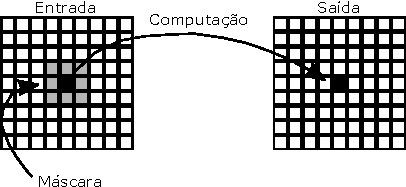
\includegraphics[width=0.7\textwidth]{figs/stencilComp.pdf}
	\caption{Ilustração do padrão estêncil oferecido pelo \pskel.}
	\label{fig:stencil}
\end{figure}



\section{\textit{Framework} PSkel}
O PSkel é um \fw de programação em alto nível para o padrão estêncil, que oferece suporte à execuções paralelas em arquiteturas heterogêneas incluindo CPU e GPU. Utilizando uma única interface de programação escrita em C++, o usuário é responsável por definir o \textit{kernel} principal da computação estêncil, enquanto o \fw se encarrega de gerar código executável para as diferentes plataformas paralelas e realizar todo o gerenciamento de memória e transferência de dados entre dispositivos de forma transparente~\cite{pereira15}.

Mais especificamente, o PSkel traduz as abstrações em código C++ de baixo nível, compatível com Intel TBB e NVDIA CUDA. Além disso, é utilizado compilação estática para o particionamnto de tarefas e dados no PSkel.

A API do PSkel possibilita a definição de \textit{templates} para a manipulação de estruturas $n$-dimensionais, denominadas \texttt{Array} (1 dimensão), \texttt{Array2D} (2 dimensões) e \texttt{Array3D} (3 dimensões). Além disso, o \fw provê abstrações para a definição da vizinhança do estêncil (\texttt{Mask}) e o \textit{kernel} da computação estêncil (\texttt{stencilKernel()}). O \texttt{stencilKernel()} é um método a ser implementado pelo usuário que descreve, especificamente, a computação que será executada para cada célula do \texttt{Array} de entrada com base nos valores de sua vizinhança (\texttt{Mask}).

Desta forma, o desenvolvedor deverá identificar a dimensão do problema, construindo estruturas de acordo com os \textit{containers} especificados pelo \fw; definir o método \texttt{stencilKernel} que descreve a computação executada sobre os elementos da máscara e do \texttt{Array} de entrada; instanciar um ou mais objetos \texttt{Stencil} para gerenciar os encapsulamentos, alocação de memória e chamadas para efetuar a computação determinada pelo \texttt{stencilKernel}. Os \textit{containers} são estruturas que armazenam \texttt{Arrays} para leitura/escrita de dados. Eles são responsáveis por gerenciar a alocação de memória na \cpu e \gpu.
Por fim, o desenvolvedor irá instanciar a classe de \textit{Runtime} que adota um padrão \textit{Facade} que abstrai os detalhes da implementação e configurações do padrão estêncil. Essa classe provê os métodos de execução para os padrões estêncil, além do particionamento transparente de tarefas e dados entre \cpu e \gpu.

% \begin{figure}[t]
% \centering
% 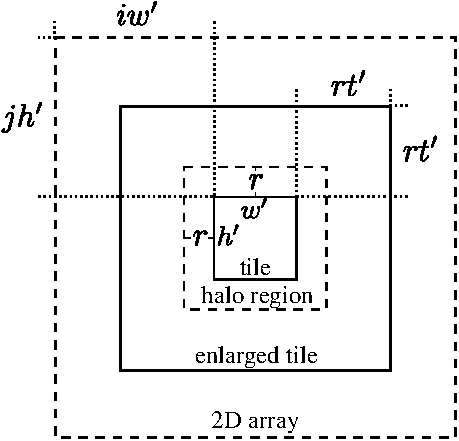
\includegraphics[width=0.3\columnwidth]{figs/tile.pdf}
% \caption{ Diagrama do \textit{tiling} 2D. Um \textit{tile} lógico (linha interna sólida) é contido dentro do Array
%     2D (linha externa pontilhada) com \textit{offsets} verticais e horizontais dado por $j  h^\prime$
%     e $i  w^\prime$. Computar $t^\prime$ consecutivas iterações estêncil no \textit{tile} requer um aumento no
%     \textit{tile} lógico com uma \textit{ghost zone} (área entre a linha interna sólida e a linha externa sólida), que é constituída
%     de regiões \textit{halo} (área entre a linha interna sólida e a linha interna pontilhada).}
% \label{fig:gputile}
% %\vspace{-4em}
% \end{figure}
%
Em uma aplicação estêncil iterativa, cada iteração utiliza a máscara de vizinhança (\texttt{Mask}) sobre o \texttt{Array} de entrada para determinar o valor de cada célula do \texttt{Array} de saída. No exemplo da Figura~\ref{fig:stencil}, o valor de cada célula do \texttt{Array} de saída é determinado em função dos valores de cada uma das células vizinhas adjacentes. Esse processo é realizado para todas as células do \texttt{Array} de entrada, produzindo um \texttt{Array} de saída da computação estêncil. Ao final de uma iteração, o \texttt{Array} de saída será considerado como \texttt{Array} de entrada para a próxima iteração no caso de uma aplicação estêncil iterativa.

No código abaixo temos um exemplo de aplicação no \fw. Nele temos a especificação do \texttt{stencilKernel} da aplicação, além das estruturas para efetuar a computação, como o \texttt{Array} de entrada e saída, a máscara da computação, entre outras estruturas.

\renewcommand{\lstlistingname}{Código}
\definecolor{lightgray}{rgb}{0.97,0.97,0.97}
\definecolor{lightred}{rgb}{1,0.7,0.7}
\lstdefinelanguage{cc}{
    language     = C++,
    morekeywords = {Array2D, __parallel__, Mask2D, Stencil2D}
}

\lstset{
numbers=none,
stepnumber=1,
numbersep=-8pt,
numberstyle=\small\color{black},
basicstyle=\scriptsize\ttfamily,
keywordstyle=\color{blue},
commentstyle=\color{black},
stringstyle=\color{black},
numberstyle=\footnotesize\ttfamily\color{black},
escapeinside={(@}{@)},
frame=none, %single
tabsize=2,
float,
language=C++, %morecomment=[l][{\color[rgb]{0.1, 0.2, 0.8}}]{},
%aboveskip=0.1in, % space before the caption
%belowskip=0.1in, % space after listing
captionpos=b,
showstringspaces=false,
%belowcaptionskip=1\baselineskip,
%breaklines=true,
%moredelim=[l][\color{blue}]{\#pragma},
backgroundcolor=\color{white},
%xleftmargin=.2\textwidth, xrightmargin=.2\textwidth
}

\begin{figure}[thp] % the figure provides the caption
\centering          % which should be centered
\begin{tabular}{c}

\begin{lstlisting}[]
(@\textcolor{blue}{\textbf{\_\_parallel\_\_}}@) void
stencilKernel((@\textcolor{blue}{\textbf{Array2D}}@)<float> A, (@\textcolor{blue}{\textbf{Array2D}}@)<float> B,
             (@\textcolor{blue}{\textbf{Mask2D}}@)<int> mask, struct Arguments args,
             int x, int y){
    B(x,y) = args.alpha * (A(x,y+1) + A(x,y-1) +
                           A(x+1,y) + A(x-1,y));
 }

void main(){
 /* ... */
 (@\textcolor{blue}{\textbf{Array2D}}@)<float> input(A,M,N);
 (@\textcolor{blue}{\textbf{Array2D}}@)<float> output(B,M,N);
 int neighbors = {{0,1}, {-1,0}, {1,0}, {-1,0}};
 (@\textcolor{blue}{\textbf{Mask2D}}@)<int> mask(4, neighbors);
 struct Arguments args(alpha, beta);
 /* ... */
 (@\textcolor{blue}{\textbf{Stencil2D}}@)<Array2D<float>, Mask2D<int>, Arguments>
             jacobi(A,B,args);
 jacobi.runIterative(device::GPU, timesteps, 1.0);
 /* ... */
}
\end{lstlisting}
\end{tabular}
\caption*{Exemplo de código no PSkel.}
\end{figure}


\section{Kalray MPPA-256}
O \mppa é um processador \textit{manycore} desenvolvido pela empresa francesa Kalray, o qual possui 256 núcleos de processamento de 400 MHz denominados \pes. Além dos PEs, o processador possui 32 núcleos dedicados a gerência de recursos denominados \textit{Resource Managers} (RMs). PEs e RMs são distribuídos fisicamente no \textit{chip} em 16 \textit{clusters} e 4 subsistemas de Entrada/Saída (E/S), contendo cada \textit{cluster} 16 PEs e 1 RM. Além dos \textit{clusters}, o \mppa possui 4 subsistemas de E/S contendo, cada um, 4 RMs. Toda a comunicação entre \textit{clusters} e/ou subsistemas de E/S é feita através de uma \noc \textit{torus} 2D. A arquitetura do \mppa pode ser vista na Figura~\ref{fig:mppa}.

A finalidade principal dos PEs é executar \textit{threads} de usuário de forma ininterrupta e não preemptível para realização de computação. PEs de um mesmo \textit{cluster} compartilham uma memória de 2 MB, a qual é utilizada para armazenar os dados a serem processados pelos PEs. Cada PE possui também uma memória \textit{cache} associativa 2-\textit{way} de 32KB para dados e uma para instruções. Porém, o processador não dispõe de coerência de \textit{caches}, o que dificulta o desenvolvimento de aplicações para esse processador. Por outro lado, a finalidade dos RMs é gerenciar E/S, controlar comunicações entre \textit{clusters} e/ou subsistemas de E/S e realizar comunicação com uma memória RAM. Na arquitetura utilizada, um dos subsistemas de E/S está conectado a uma memória externa \lpddr de 2 GB.

\begin{figure}[t]
	\centering
	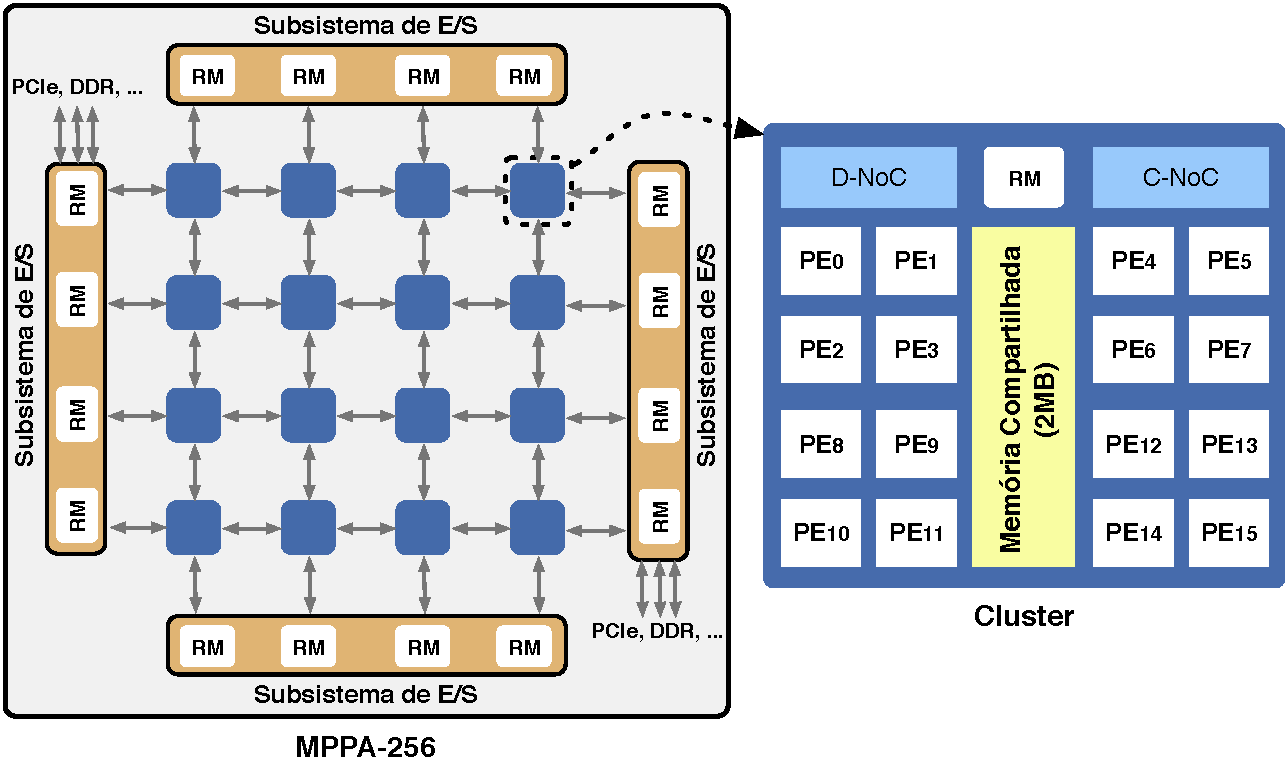
\includegraphics[width=0.7\textwidth]{figs/mppa-overall.pdf}
	\caption{Visão geral do \mppa.}
	\label{fig:mppa}
\end{figure}


Trabalhos anteriores mostraram que desenvolver aplicações paralelas otimizadas para o \mppa é um grande desafio~\cite{Castro-IA3-JPDC:2014} devido a alguns fatores importantes. O primeiro deles está relacionado ao \textbf{modelo de programação híbrido} exigido pelo processador: \textit{threads} em um mesmo \textit{cluster} se comunicam através de uma memória compartilhada local, porém a comunicação entre \textit{clusters} é feita explicitamente via \noc, em um modelo de memória distribuída. Mais especificamente, aplicações desenvolvidas para o \mppa precisam utilizar duas bibliotecas de programação paralela para utilizar os recursos do processador: OpenMP, baseado em um modelo de memória compartilhada, utilizada para paralelizar a computação dentro de cada \textit{cluster} e uma \api proprietária, que segue um modelo de memória distribuída, sendo utilizado na comunicação entre os \textit{clusters} e o subsistema de E/S por meio da NoC. O segundo fator importante está relacionado a \textbf{capacidade limitada de memória} no \textit{chip}: cada \textit{cluster} possui apenas 2 MB de memória local de baixa latência. Portanto, aplicações reais precisam constantemente realizar comunicações com o subsistema de \io conectado à memória \lpddr. Por fim, o último fator está diretamente relacionado à \textbf{ausência de coerência de \textit{cache}}: cada \pe possui uma memória \textit{cache} privada sem coerência de \textit{cache}, sendo necessário o uso explícito de instruções do tipo \textit{flush} para atualizar a \textit{cache} de um \pe quando necessário.

